\chapter{Domain Driven Design}
In diesem Kapitel wird die Ubiquitous Language unseres Projektes analysiert. Außerdem werden die Entities \& Value Objects basierend auf der entwickelten Software modelliert und abschließend die verwendeten Repositories und Aggregates analysiert und erklärt.
\section{Ubiquitous Language}
\subsection{Sprache}
Ubiquitous Language  bedeutet, eine Sprache und die Begriffe so zu wählen, dass die Domänenexperten und die Entwickler minimalen Übersetzungsaufwand haben.  Aufgrund einer deutschen Domäne und Anwendung haben wir deutsche Domänen Begriffe verwendet.
Die Dateinamen und Ordner der Javaklassen wurden so gewählt, dass sie den Domänenexperten und den Nicht-Entwicklern mit kurzen und aussagekräftigen Worten Aufschluss über die Funktionalität geben.
Da sich Ubiquitous Language  auf das gesamte Projekt bezieht, wurden auch die Tests in der Domain Sprache geschrieben und sollen für alle Leser verständlich sein. Der Test \href{https://github.com/MichaelaHaag/RezeptApp/blob/main/3-Domain-Code/src/test/java/de/rezeptapp/domain/Rezept/RezeptRepositoryTest.java}{\code{RezeptReositoryTest}}, repräsentiert sehr gut die verwendete Ubiquitous Language.
\subsection{Begriffsdefinition}
Die Anwendungsdomäne befasst sich mit der Verwaltung von Rezepten. Daher ist der erste zentrale Begriff der Domäne das \textbf{Rezept}. Ein Rezept setzt sich aus einer ID, einem Titel, einer Beschreibung, einer Menge von \textbf{Zutaten}, einer Menge von Rezept \textbf{Kategorien}, einer \textbf{Schwierigkeit} und optional einem \textbf{Bild} zusammen. Eine \textbf{Zutat} enthält Informationen über den Namen der Zutat, in welcher \textbf{Menge} die Zutat in das Rezept gehört, sowie die dazugehörende \textbf{Einheit}. Die \textbf{Einheit} setzt sich aus einem Namen und einer Beschreibung zusammen.
Ein weiterer wichtiger Begriff in der Domäne sind die Rezept \textbf{Kategorien}. Sie enthalten einen Namen, eine Beschreibung und zusätzlich noch eine Kurzform des Namens für eine schönere Visualisierung in der Benutzeroberfläche.
Die \textbf{Schwierigkeit} eines Rezeptes kann in der Domäne \textbf{einfach}, \textbf{mittel} oder \textbf{schwer} sein. Das \textbf{Bild} enthält neben dem Verweis auf das zugehörige Rezept noch den \textbf{Pfad}, unter dem das Bild gespeichert ist.
\section{Entities \& Value Objects}
In diesem Unterkapitel werden wir die Entities und Value Objects in unserer Rezepte-Anwendung genauer analysieren. Entities sind Objekte, die eine Identität haben. Sie haben eine eindeutige ID und können von anderen Objekten referenziert werden. In unserer Anwendung haben wir verschiedene Entities. In \autoref{fig:RepositoriesUML} sind die Entities in Blau dargestellt.

\code{Rezept} ist eine Entity, da es eine eindeutige Identität und veränderliche Eigenschaften hat. Ein Nutzer kann in der Anwendung die Rezepte nach dem Erstellen immer wieder bearbeiten. Die \code{Zutaten} eines Rezepts setzen sich aus einer Menge, dem Namen der Zutat, einer ID und der ID des zugehörigen Rezepts zusammen. Außer den beiden IDs können auch die Eigenschaften von Zutaten verändert werden. Daher ist auch die Zutat ein Entity. Das \code{Bild}, das zu einem Rezept gehört, wird in unserer Anwendung auch als Entity betrachtet, da es eindeutig identifizierbar ist, durch eine eindeutige ID mit dem Rezept verknüpft werden kann und über die Eigenschaft Pfad verfügt. Der Pfad des Bildes kann verändert werden. \code{Kategorie} ist die vierte Entity der Domäne. Rezepte werden verschiedenen Kategorien zugeordnet und die Nutzer können sich eine Liste mit allen Rezepten für eine Kategorie anschauen, dafür ist es notwendig, dass Kategorie eine eindeutige ID hat und referenzierbar ist.

Value Objects hingegen haben keine Identität. Sie werden lediglich durch ihre Eigenschaften definiert und können nicht von anderen Objekten referenziert werden. In \autoref{fig:RepositoriesUML} sind die Value Objects in Rosa dargestellt. In unserer Anwendung gibt es das Value Object: \code{Menge}. Eine Zutaten-Menge hat keine eindeutige Identität, sondern beschreibt einfach den Umfang oder die Menge einer bestimmten Zutat, die in einem Rezept verwendet wird. Eine Zutaten-Menge hat keine eigenen Eigenschaften oder Verhaltensweisen und kann nicht auf andere Objekte referenzieren. Die Menge setzt sich aus einer Zahl und einer Einheit zusammen. 

In der Domäne gibt es zusätzlich die Enumerationen \code{Schwierigkeit} und \code{Einheit}. Enumerationen können eine Sammlung von Value Objects sein, wenn in den Enum-Instanzen kein veränderbarer Zustand hinterlegt ist. Die Enumeration \code{Schwierigkeit} kann nur die Werte: \emph{Einfach}, \emph{Normal} und \emph{Schwer} annehmen und diese Instanzen haben keine Member-Felder und sind nicht veränderbar. Darum handelt es sich bei dem Enum Schwierigkeit um ein Value Object. Bei der Enumeration \code{Einheit} ist das ähnlich. Einheit hat keine eindeutige Identität und beschreibt lediglich die Art der Messung, die verwendet wird, um die Menge einer Zutat zu beschreiben, z.B. Gramm oder Teelöffel. Es hat allerdings die Member-Felder Name und Beschreibung. Daher wird die Einheit, die bei der Angabe der Menge einer Zutat verwendet wird, als Entity betrachtet.

Wir haben uns dazu entschieden, die ID bei allen Entities mit Surrogatschlüsseln umzusetzen. Dafür haben wir allen Entity Elementen in unserer Domäne eine UUID gegeben. Universally Unique Identifier, kurz UUID, ist ein Standard für Identifikationsnummern. Vorteile von UUIDs sind, dass sie jederzeit generierbar sind und dass sie anwendungsübergreifend eindeutig sind. Außerdem ist hier die Verteilung der IDs einfacher, da eine UUID generiert werden kann, ohne dass sie mit den bereits vorhandenen UUIDs verglichen werden muss, da es sehr unwahrscheinlich ist, dass versehentlich doppelte UUIDs generiert werden. Die Nachteile, wie: nicht sprechend, keine Bedeutung in der Domäne und eventuelle Engpässe bei Generierung in
Hochlastsystemen sind in unserer Anwendung nicht von Bedeutung, da der Schlüssel einfach aus der CSV-Datei ausgelesen werden kann.

\section{Aggregates}
Aggregate gruppieren die Entities und Value Objects zu gemeinsam verwalteten Einheiten. Die Verwendung von Aggregaten ermöglicht das Entkoppeln der Objektbeziehungen, das Bilden natürlicher Transaktionsgrenzen und die kontinuierliche Übereinstimmung mit den Domänenregeln.
Alle Klassen im Paket \href{https://github.com/MichaelaHaag/RezeptApp/tree/main/3-Domain-Code/src/main/java/de/rezeptapp/domain/Rezept}{\code{Rezept}} bilden Eigenschaften eines Rezeptes ab, daher werden diese zu einem Aggregate zusammengefasst. Dazu gehören Rezept, Kategorie, Bild und Schwierigkeit. Die Root Entität ist dabei das Rezept selbst. Im zweiten Aggregat befindet sich nur die \href{https://github.com/MichaelaHaag/RezeptApp/tree/main/3-Domain-Code/src/main/java/de/rezeptapp/domain/Kategorie}{\code{Kategorie}}, da die Kategorien eigen verwaltet werden. \autoref{fig:RepositoriesUML} zeigt die Aufteilung der Aggregate in die beiden Ordner. 

\section{Repositories}
Für den Zugriff auf den persistenten Speicher werden zwei Repositories gemäß dem Grundsatz „Ein Repository pro Aggregat“ definiert: Das \href{https://github.com/MichaelaHaag/RezeptApp/tree/main/3-Domain-Code/src/main/java/de/rezeptapp/domain/Rezept/RezeptRepository.java}{\code{RezeptRepository}} erlaubt den Zugriff auf das Rezept, also die Root Entity des entsprechenden Aggregates (siehe \autoref{fig:RepositoriesUML}). Analog hierzu ermöglicht das \href{https://github.com/MichaelaHaag/RezeptApp/blob/main/3-Domain-Code/src/main/java/de/rezeptapp/domain/Kategorie/KategorieRepository.java}{\code{KategorieRepository}} Zugriff auf die Kategorie als Root Entity des zugehörigen Aggregates (siehe \autoref{fig:RepositoriesUML}). Die Repositories enthalten spezifische Methoden des \code{EntityManagers} zur Speicherung. Im RezeptReposetory werden die Daten in drei verschiedenen CSV-Dateien gespeichert. Dafür gibt es verschiedene Gründe. Die Zutaten mit den jeweiligen Eigenschaften werden separat voneinander gespeichert, da hier eine 1:n Beziehung herrscht und wir hier Redundanz der Daten vermeiden wollen. In der CSV-Datei für die Zutaten wird daher die ID des jeweiligen Rezeptes mitgespeichert. Bei den Bildern eines Rezeptes ist das ähnlich. Auch hier herrscht eine 1:n Beziehung. Zusätzlich haben wir uns für eine getrennte Speicherung zur besseren Organisation entschieden. 

\begin{figure}[ht]
	\centering
	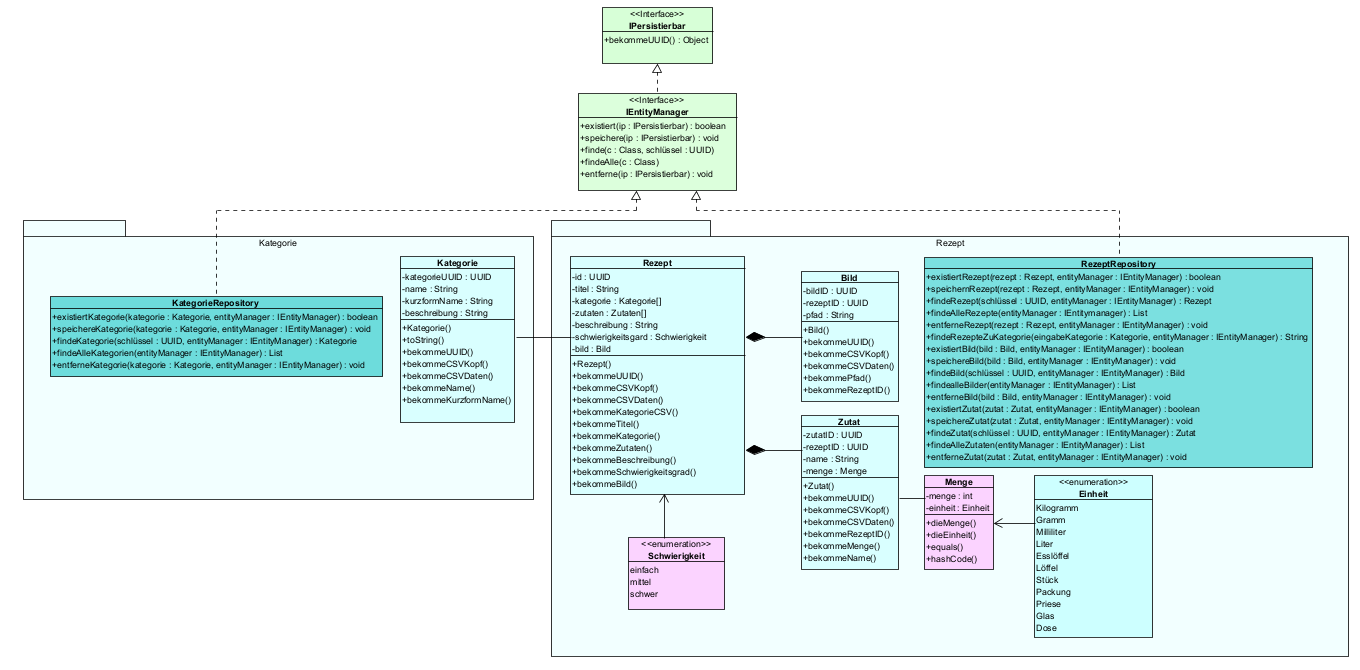
\includegraphics[width=1.0\textwidth]{Bilder/Reposetory-UML.png} 
	\caption{UML-Diagramm Repositories}
	\label{fig:RepositoriesUML}
\end{figure}
